\documentclass{problemset}
\usepackage{amsmath}

\usepackage{lipsum}
%\usepackage{showframe}
\usepackage{layout}


\usepackage[charter,cal=cmcal]{mathdesign} %different font
\usepackage{microtype}
\usepackage{amsmath}
%\usepackage{amsfonts}
%\usepackage{amssymb}
\usepackage{graphicx}
\usepackage[inline]{enumitem}
\usepackage{xparse}
\usepackage{ifthen}
\usepackage{graphicx}
\usepackage{caption}
\usepackage{subcaption}
\usepackage{kbordermatrix}
\usepackage{color}
\usepackage{tikz}
\usepackage{fancyhdr}
\usepackage{calc}
\usepackage[hidelinks]{hyperref}

\usepackage{pgfplots}
\pgfplotsset{compat=newest}
\usetikzlibrary{automata,arrows,positioning,calc}
%%%
% Useful Linear Algebra macros
%%%
\newcommand{\ul}{$\underline{\phantom{xxx}}$}
\newcommand{\ull}{\underline{\phantom{xxx}}}
\newcommand{\xh}{{\hat {\mathbf x}}}
\newcommand{\yh}{{\hat {\mathbf y}}}
\newcommand{\zh}{{\hat {\mathbf z}}}
\newcommand{\R}{\mathbb{R}}
\newcommand{\Z}{\mathbb{Z}}
\newcommand{\N}{\mathbb{N}}
\newcommand{\E}{\mathbb{E}}
\newcommand{\proj}{\mathrm{proj}}
\newcommand{\Proj}{\mathrm{proj}}
\newcommand{\Perp}{\mathrm{perp}}
\renewcommand{\span}{\mathrm{span}\,}
\newcommand{\Span}{\mathrm{span}\,}
\newcommand{\Img}{\mathrm{img}\,}
\newcommand{\Null}{\mathrm{null}\,}
\newcommand{\Range}{\mathrm{range}\,}
\newcommand{\rref}{\mathrm{rref}}
\newcommand{\rank}{\mathrm{rank}}
\newcommand{\Rank}{\mathrm{rank}}
\newcommand{\nnul}{\mathrm{nullity}}
\newcommand{\mat}[1]{\begin{bmatrix}#1\end{bmatrix}}
\newcommand{\chr}{\mathrm{char}}
\renewcommand{\d}{\mathrm{d}}
\renewcommand{\P}{\mathbb{P}}
\newcommand{\ldsto}{\underset{\text{\tiny leads to}}{\leadsto}}

\newcommand{\fatrule}[1]{\vspace{.3cm}\hrule {\hfill \sf #1}}

%\tcbuselibrary{skins}
%\usetikzlibrary{shadings}

%\definecolor{defcolor}{rgb}{.05,.4,.15}
%\colorlet{defframecolor}{green!50!black}
\declareoutlinedbox{lemma}{LEMMA}{LEM}{defframecolor}{defcolor}
\declareoutlinedbox{corollary}{COROLLARY}{COR}{defframecolor}{defcolor}
\newenvironment{proof}{\emph{Proof.}}{\hfill$\square$}
%%%
% Set up the margins to use a fairly large area of the page
%%%
\textwidth=6in
\topmargin=-1in
\textheight=10in
\parskip=.07in
\parindent=0in

\begin{document}
%\pagestyle{empty}
\pagestyle{fancy}
\rfoot{\footnotesize\it \copyright\,Jason Siefken, 2016 \ \makebox(30,5){\includegraphics[height=1.2em]{by-sa.pdf}}}
\renewcommand{\headrulewidth}{0pt}

\begin{center}
	{\huge\bf Introduction to Stochastic Processes \\{\sc Math 310-2}}\\

\vspace{.7in}
{
\it \copyright\,Jason Siefken, 2016 \\
Creative Commons By-Attribution Share-Alike\, \makebox(30,5){\includegraphics[height=1.2em]{by-sa.pdf}}
}
\end{center}

\section*{Introduction}


	In Math 310-1, you studied random variables and sequences of random variables that
	were \emph{independent}.  Because they were independent, they satisfied properties like 
	the central limit theorem and the law of large numbers.

	But, many worldly phenomena are not independent.  In this class
	we will study a basic type of non-independent process---Markov chains.

	\begin{definition}[Markov Chain]
		A sequence of random variables $(X_n)$ is a \emph{Markov chain} (or
		Markov for short) if for $n$ and any sequence of events $(A_i)$ having positive
		probability,
		\[
			\P(X_n\in A_n \mid X_{n-1}\in A_{n-1}) = \P(X_n\in A_n\mid X_{n-1}\in A_{n-1},X_{n-2}\in A_{n-2},\ldots).
		\]
	\end{definition}

	In other words, $(X_n)$ is \emph{Markov} if knowing the previous value in the sequence
	gives you the same amount of information as knowing all previous values.  Since we will be looking
	at conditional probabilities a lot, to keep things less cluttered, we will sometimes
	avoid writing the events.  That is,
	\[
		\P(X_n\in A_n\mid X_{n-1}, X_{n-2},\ldots) \equiv \P(X_n\in A_n| X_{n-1}\in A_{n-1}, X_{n-2}\in A_{n-2},\ldots)
	\]
	where $(A_i)$ is a sequence of positive probability events.  Further, $\P(X_n)$, will mean the distribution of $X_n$.

	Let's look at some sequences and decide whether or not they are Markov.


	\begin{enumerate}
		\item You're walking around Chicago.  At each street intersection, you
			roll a die to decide which street to go down next.
			$(X_n)$ is the sequence of streets you walk down.
			\begin{quote}
				Markov!  The next street you decide to go down depends only
				on your current position, not on how you got there.
			\end{quote}
		\item You're trying to hack a computer network.  Every minute you have a $50\%$ chance
			to crack another password.  If you've cracked $k/2$ passwords in the last $k$ minutes, 
			your heart-rate gets high, otherwise it is normal.  $(X_i)$ is your heart-rate
			in the $i$th minute.
			\begin{quote}
				Markov, but not \emph{stationary}.  For minute $n$, if you are
				told that $X_{n-1}=$caught, you know with probability 1 that $X_n$ will
				be caught.  Alternatively, if you're told $X_{n-1}=$not caught, you know
				that $X_{n-2},\ldots=$not caught, and so you get know extra information
				knowing all previous states.
			\end{quote}
		\item You're trying to hack a computer network.  Every minute you have a $50\%$ chance
			to crack another password.  If you crack $k$ passwords, 
			you will be discovered.  $(X_i)$ is how many passwords you've
			cracked by the $i$th minute.
			\begin{quote}
				Markov! If you've cracked $n$ passwords in the $i$th minute, 
				you still have a 50/50 chance of cracking your $(n+1)$th password in the $(i+1)$th
				minute, regardless of whether you cracked $n$ or $n-1$ in the $(i-1)$th minute.
			\end{quote}
		\item $(X_i)$ is an independent and identically distributed (iid) sequence of Bernoulli
			$(1/3,2/3)$ random variables.
			\begin{quote}
				Markov!  We trivially have $\P(X_i\mid X_{i-1}) = \P(X_i) = \P(X_i\mid X_{i-1}, X_{i-2},\ldots)$ by independence.
			\end{quote}
		\item You repeatedly take a test to become part of your favorite fan club.  $(X_i)$ is your average 
			score on the first $i$ tests.
			\begin{quote}
				Markov, but not \emph{stationary}.  This one is subtle.  Suppose that your
				score on the $i$th test is given by the independent sequence $S_i$.  Then
				\[
					X_i = \tfrac{1}{n}\sum_{n=1}^i S_i.
				\]
				We then have $\P(X_i=a\mid X_{i-1}=b) = \P\left(\frac{S_i+(i-1)b}{i} = a\right)$.  Since $S_i$ 
				is an independent sequence, knowing $X_{i-2}$ doesn't change this probability.
			\end{quote}
	\end{enumerate}

	\fatrule{Day 2}

	\subsubsection*{Notation}

	Let $(X_i)$ have the Markov property. We call the codomain$(X_i)=X^{(i)}$ the \emph{state space}, and we will
	assume $X^{(i)}=X^{(j)}$.

	$\P(X_i=b\mid X_{i-1}=a)$ is called the \emph{transition probability} from state $a$ to state $b$ at time $i$.  If
	\[
		\P(X_i=b\mid X_{i-1}=a) = \P(X_j=b\mid X_{j-1}=a)\qquad \text{for all }i\text{ and }j,
	\]
	we call $(X_i)$ \emph{stationary}.  We will only consider stationary processes.


	For a stationary process $(X_i)$,
	\[
		P(a,b) \equiv \P(X_i=b\mid X_{i-1}=a)\qquad \text{and}\qquad P^n(a,b) \equiv \P(X_i=b\mid X_{i-n}=a)
	\]
	are called the \emph{one-step transition function} and the \emph{multi-step transition function}.

	\subsection*{A Simple Example}


	Your very conservative aunt decided to go to a Chicago comedy club.  Each joke leaves her happy ($H$)
	or angry ($A$).  If she is happy, the next joke has a 50/50 chance of leaving her happy or angry.
	If she is angry, the next joke has a $1/4$th chance of making her happy and a $3/4$ths chance
	of making her angry.

	\fatrule{Day 3}

	We can model this situation with a directed graph:

	\begin{center}
	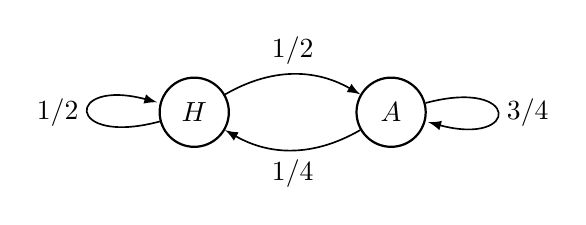
\begin{tikzpicture}[>=latex,scale=2.5,auto,semithick,node distance=3cm]
	\tikzstyle{every state}=[fill=white,draw=black,thick,text=black,scale=1]

	\tikzset{vertex/.style = {shape=circle,draw,minimum size=1.5em}}
	\tikzset{edge/.style = {->}}
	% vertices
	\node[state] (H) at  (0,0) {$H$};
	\node[state] (A) at  (1,0) {$A$};
	%edges
	\path (H) edge[->,bend left] node {$1/2$} (A) ;
	\path (A) edge[->,bend left] node {$1/4$} (H) ;
	\path (A) edge[->,loop right] node {$3/4$} (A) ;
	\path (H) edge[->,loop left] node {$1/2$} (H) ;

	\end{tikzpicture}
	\end{center}

	\begin{definition}
		The \emph{transition matrix} associated with a stationary Markov chain $(X_i)$ having
		$n$ states $\{1,2,\ldots, n\}$ is the matrix $T=[t_{ij}]$ where $t_{ij}=P(i,j)$.
	\end{definition}

	For this example, letting happy be the first state and angry be the second state, we have
	\[
		T=\kbordermatrix{& H & A\\ H &\P(H\to H) & \P(H\to A)\\ A &\P(A\to H) & \P(A\to A)}=\mat{1/2&1/2\\1/4&3/4}.
	\]
	Let's compute $P^2(A,A)=\P(X_i=A\mid X_{i-2}=A)$.  There are only two ways for this to happen.  Either
	the states went 
	\[
		A\to A\to A\qquad\text{or}\qquad A\to H\to A.
	\]
	$\P(A\to A\to A) = \frac{3}{4}\cdot \frac{3}{4} = \frac{9}{16}$ and $\P(A\to H\to A) = \frac{1}{4}\cdot \frac{1}{2}=\frac{2}{16}$,
	and so
	\[
		P^2(A,A) = \P(A\to A\to A)+\P(A\to H\to A) = \frac{11}{16}.
	\]

	The $P^2$ transition matrix now looks like $\mat{?&?\\?&\frac{11}{16}}$.  Computing every
	entry we get $\mat{\frac{6}{16}&\frac{10}{16}\\\frac{5}{16}&\frac{11}{16}}$.


	Let's look at what happened from a matrix perspective:  To compute $P^2(A,A)$, we
	need to compute the quantity $Q=\P(A\to A\to A)+\P(A\to H\to A)$, and by the 
	Markov property,
	\[
		\P(A\to A\to A) =  \P(A\to A)\P( A\to A)
		\qquad\text{and}\qquad
		\P(A\to H\to A) =  \P(A\to H)\P( H\to A).
	\]
	If we squint, we see
	\[
		Q=\mat{\P( H\to A)\\ \P(A\to A)}\cdot \mat{\P(A\to H)\\\P(A\to A)}
		=\mat{\P( H\to A) & \P(A\to A)} \mat{\P(A\to H)\\\P(A\to A)}
		=(\mat{0&1}T)\left(T\mat{0\\1}\right) = \mat{0&1}T^2\mat{0\\1}.
	\]

	In other words, the $(2,2)$ entry of the transition matrix for $P^2(x,y)$ is the
	$(2,2)$ entry of $T^2$.  In fact, the transition function $P^2(x,y)$ is given by the
	matrix $T^2$!

	Using induction, we can show that the transition function $P^n(x,y)$ is given by
	the matrix $T^n$ for any $n$, but first let's prove a lemma we've already used once.

	\begin{lemma}
		If $(X_i)$ is a Markov chain and $(s_i)$ is a sequence of states of $(X_i)$, then
		\[
			\P(s_1\to s_2\to\cdots \to s_n) = \prod_{i=1}^{n-1} \P(s_i\to s_{i-1}).
		\]
	\end{lemma}
	
	We used this lemma already when we said $\P(A\to H\to A) = \P(A\to H)\P(H\to A)$,
	and it seems quite intuitive given the definition of Markov.

	\begin{proof}
		We will proceed by induction.  Trivially, $\P(s_1\to s_2) = \P(s_1\to s_2)$.
		Suppose $\P(s_1\leadsto s_n) = \prod \P(s_i\to s_{i+1}$, and consider
		$\P(s_1\leadsto s_n\to s_{n+1})$.  By definition
		\[
			\P(s_n\to s_{n+1}) = \P(X_{n+1}=s_{n+1}\mid X_{n}=s_{n}) 
		\]\[
			= \P(X_{n+1}=s_{n+1}\mid X_{n}=s_{n}, X_{n-1}=s_{n-1}, \ldots)
		\]
		with the last equality following from the Markov property.  Now by the definition
		of conditional probability we have
		\[
			\P(X_{n+1}=s_{n+1}\mid X_{n}=s_{n}, X_{n-1}=s_{n-1}, \ldots)
			=\frac{\P(X_{n+1}=s_{n+1}, X_{n}=s_{n}, X_{n-1}=s_{n-1}, \ldots)}{
			\P(X_{n}=s_{n}, X_{n-1}=s_{n-1}, \ldots)} = \frac{\P(s_1\leadsto s_n\to s_{n+1})}{\P(s_1\leadsto s_n)}.
		\]
		Multiplying both sides by $\P(s_1\leadsto s_n)$ gives us
		\[
			\P(s_1\leadsto s_n\to s_{n+1})
			=\P(s_1\leadsto s_n)\P(s_n\to s_{n+1}).
		\]
		Since we assume that $\P(s_1\leadsto s_n)$ could be written as a product, we've completed the proof.
	\end{proof}

	\fatrule{Day 4}

	We're almost ready to tackle our first theorem, but let's first prove two more
	easy facts.

	\begin{lemma}
		If $(X_i)$ is a Markov chain with finite state space $S$, then 
		\[
			\P(X_n=b) = \sum_{s\in S} \P(X_n=b\mid X_{n-1}=s)\P(X_{n-1}=s).
		\]
	\end{lemma}

	\begin{proof}
		Since $\P(X_i\in S)=1$, we have
		\[
			\P(X_n=b) = \P(X_n=b\text{ and } X_{n-1}\in S)=\P\left(\bigcup_{s\in S} X_n=b\text{ and } X_{n-1}=s\right).
		\]
		Since the events $(X_n=b\text{ and } X_{n-1}=s)$ and $(X_n=b\text{ and } X_{n-1}=s')$ are disjoint if $s\neq s'$,
		we have
		\[
			\P\left(\bigcup_{s\in S} X_n=b\text{ and } X_{n-1}=s\right)
			=
			\sum_{s\in S} \P(X_n=b\text{ and } X_{n-1}=s).
		\]
		Noticing the summand is just $\P(X_n=b\mid X_{n-1}=s)\P(X_{n-1}=s)$ completes the proof.
	\end{proof}

	\begin{lemma}
		If $(X_i)$ is a Markov chain with finite state space $S$, then $\P(X_n=b \mid X_1=a)$ is the sum
		of $\P(a\to s_2\to s_3\to\cdots \to s_{n-1}\to b)$ for every possible
		combination of $s_2,\ldots ,s_{n-1}\in S$.
	\end{lemma}

	\begin{proof}
		Like the previous proof, this follows from manipulations of the basic definitions.

		First note, if $s_2,\ldots, s_{n-1}$ and $s_2',\ldots, s_{n-1}'$ are not the exact
		same sequence, then the events $a\to s_2\to \cdots \to s_{n-1}\to b$ and
		$a\to s_2'\to \cdots \to s_{n-1}'\to b$ are disjoint.  Thus
		\[
			\P\left(\bigcup_{s_2,\ldots,s_{n-1}\in S} a\to s_2\to \cdots \to s_{n-1}\to b\right) = 
			\sum_{s_2,\ldots,s_{n-1}\in S} \P(a\to s_2\to \cdots \to s_{n-1}\to b).
		\]
		Now, by the definition of conditional probability,
		\[
			\P(a\to s_2\to \cdots \to s_{n-1}\to b) = \frac{\P(X_1=a, X_2=s_2,\ldots, X_{n-1}=s_{n-1},X_n=b)}{\P(X_1=a)},
		\]
		and so
		\[
			\P\left(\bigcup_{s_2,\ldots,s_{n-1}\in S} a\to s_2\to \cdots \to s_{n-1}\to b\right)
			=\frac{\P(X_1=a, X_2\in S,\ldots, X_{n-1}\in S,X_n=b)}{\P(X_1=a)} = \frac{\P(X_1=a, X_n=b)}{\P(X_1=a)},
		\]
		with the last equality following because  $X_i\in S$ always.  The right side of this equation
		is just $\P(X_n=b\mid X_1=a)$, and so combining all of our equations proves the result.
	\end{proof}


	Now we're ready to tackle our theorem linking matrix multiplication and multi-step transition
	functions.
	
	\begin{theorem}
		For a Markov chain $(X_i)$ having states $\{1,\ldots d\}$ and transition function $P(x,y)$,
		let $T$ be the corresponding transition matrix.  Then, the transition matrix corresponding 
		to the multi-step transition function $P^n(x,y)$ is $T^n$.
	\end{theorem}

	\begin{proof}
		We will proceed by induction.  
		By definition, $T$ gives the transition probabilities for $P(x,y)$.
		Suppose that $T^{n-1}$ gives the transition probabilities for $P^{n-1}(x,y)$.  Since
		$(X_i)$ is a Markov processes, 
		\[
			\P(s_1\leadsto s_{n-1}\to s_n) = \P(s_1\leadsto s_{n-1})\P(s_{n-1}\to s_n),
		\]
		where $s_1,\ldots, s_n$ are states.  Further, from our previous lemmas,
		\[
			\P(X_n=s_n\mid X_1=s_1) = \sum_{s\in S} \P(X_n=s_n\mid X_{n-1}=s_{n-1})\P(X_{n-1}=s_{n-1}\mid 
			X_1=s_1) 
		\]\[
			= \sum_{s\in S} P(s,s_n)P^{n-1}(s_1,s)
			= \sum_{s\in S} P^{n-1}(s_1,s)P(s,s_n).
		\]
		However, the right hand side is the same as the dot product of the $s_n$ column of $T$ with the
		$s_1$ row of $T^{n-1}$, which is the definition of the $(s_1,s_n)$ entry of $TT^{n-1}=T^n$.
	\end{proof}

	Now we know how to analyze transition probabilities for 
	any finite-state Markov chain using matrices!

	Let's see how our probability questions become linear algebra questions.  Suppose we'd like
	to know the distribution after one joke supposing that your aunt started happy.  That
	is, we'd like to know $f(x) = P(H,x)$.  This is just the first row of $T$, and so the distribution
	is given by $\mat{1&0}T$.  The distribution after $4$ steps supposing your aunt started off
	angry is $\mat{0&1}T^7$.  And $P^7(A,H)$ is $\mat{0&1}T^7\mat{1\\0}$.

	But we can do more.  Suppose we wanted to know the distribution after one joke supposing that
	there was a 50/50 chance your aunt came into the club happy or angry.  That's just 
	$\mat{1/2&1/2}T$.  In general, if $\vec d$ is a \emph{row vector} specifying an initial
	distribution, then $\vec dT^n$ gives the resulting distribution after $n$ steps.

	\fatrule{Day 5}

	Consider now the following questions: After many many jokes, what is the probability that your aunt
	leaves the club happy?  What's the probability she leaves angry?  Does the state she comes into the club
	with affect these probabilities?  How does the number of jokes told affect these probabilities?

	We can answer all of these questions with linear algebra!  Since we're going to be computing large
	powers of $T$, let's diagonalize it.

	\[
		T = \mat{1/2&1/2\\ 1/4 & 3/4} =
		\mat{-2& 1\\ 1& 1} \mat{1/4 & 0\\ 0& 1}\mat{-1/3 & 1/3 \\ 1/3& 2/3} = SDS^{-1}.
	\]

	Since $(1/4)^n\to 0$ as $n\to \infty$, we can easily compute
	\[
		T^\infty\equiv \lim_{n\to\infty} T^n = 
		\mat{-2& 1\\ 1& 1} \mat{0 & 0\\ 0& 1}\mat{-1/3 & 1/3 \\ 1/3& 2/3} = \mat{1/3&2/3\\1/3&2/3}.
	\]
	From this we can see $\mat{1 & 0}T^\infty = \mat{0&1}T^\infty$ and so her chances of being
	happy or angry upon leaving the club after many jokes doesn't depend on her initial state.  In
	either case, she leaves happy with a $1/3$ chance and angry with a $2/3$ chance.  We can also conclude
	that the number of jokes told doesn't really matter as long as the number is large.
	Indeed
	\[
		T^n-T^m = S(D^n-D^m)S^{-1} = S\mat{ \frac{1}{4^n}-\frac{1}{4^m} & 0 \\0 & 0}S^{-1}.
	\]
	As long as $n$ and $m$ are large, $\frac{1}{4^n}-\frac{1}{4^m}\approx 0$, and so the difference is
	approximately the zero matrix.

	\fatrule{Day 6}

	\subsection*{Hitting Times}

	Consider a Markov chain for a gambler.  The state space would be $\$d\geq 0$.  If the gambler has any money,
	he can bet it and transition to a state with more money or a state with less money.  But, if the gambler 
	ever has \$0, he cannot bet any further.

	The \emph{Gambler's Ruin} problem asks, how long does it take to end up in state \$0?

	\begin{definition}[Hitting Time]
		Let $(X_i)$ be a Markov chain.  A \emph{hitting time} for an event $B$ is the random
		variable 
		\[
			T_B = \min\{i\geq 0: X_i\in B\}.
		\]
	\end{definition}

	We will not compute hitting times right now, but hitting times give us another way to think
	about Markov chains.  For example,
	\[
		P^n(x,y) = \sum_{m\leq n} P(T_{\{y\}}=m\mid X_1=x)P^{n-m}(y,y).
	\]
	(Why is this formula intuitive?)

	\subsection*{Different Types of States}

	Consider the gambler's ruin problem.  If $a,b>0$, there's a non-zero chance
	of starting at state $a$ and ending at state $b$.  (Is the correct way to
	mathematical quantify this statement $P(a,b)>0$?)  However, $P^n(0,b)=0$ unless $b=0$.
	That is, you cannot transition out of state $\$0$.

	\begin{definition}[Absorbing]
		A state $a$ of a Markov chain is called \emph{absorbing} if
		$P(a,b)=0$ whenever $b\neq a$.
	\end{definition}

	In plain language, a state is absorbing if once
	you enter it, you can never leave.

	For a Markov chain, define
	\[
		\rho_{xy} = \P(T_{\{y\}} < \infty\mid X_1=x).
	\]
	That is, $\rho_{xy}$ is the probability you end up at state $y$ at some
	time in the future having started at state $x$.

	\begin{definition}[Recurrent \& Transient]
		For a Markov chain $(X_i)$, a state $a$ is called \emph{recurrent}
		if $\rho_{aa}=1$, otherwise it is called \emph{transient}.
	\end{definition}


	What are the transient and recurrent states for the gambler's ruin problem?  Well, the
	state \$0 is absorbing, and if the odds are in the house's favor, $\rho_{x0}=1$.  That
	is, you will always eventually end up at $\$0$.  Thus, the state \$0 is recurrent.  However,
	if you start at state $\$d>0$, there is a positive probability you end up at
	state \$0, and so $\rho_{dd}<1$.  This means that every state $\$d>0$ is transient.

	Now we get to our first big theorem.

	\begin{theorem}
		Let $(X_i)$ be a Markov chain, let $N(x)$ be the number of times state
		$x$ is visited, and let $G(y,x)=\E(N(x)\mid X_0=y)$. Then,
		\begin{enumerate}[label=(i)]
			\item if $x$ is recurrent, $\P(N(x) = \infty\mid X_1= x)=1$ and $G(x,x)=\infty$, and
			\item if $x$ is transient, $\P(N(x) < \infty\mid X_1=y)=1$ and
				\[
					G(y,x) = \frac{\rho_{yx}}{1-\rho_{xx}}.
				\]
		\end{enumerate}
	\end{theorem}
	In plain words, the theorem says that recurrent states are visited infinitely
	often and transient states are visited finitely often.  Also, we can precisely
	compute the expectation of the number of times a transient state is visited
	in terms of $\rho$.

	\fatrule{Day 7}


	\begin{proof}
		(i).  Suppose $x$ is a recurrent state.  Let $T^{(n)}_{\{x\}}= \min\{i > n:X_i=x\}$
		be the first return time to $\{x\}$ after time $n$.
		Since $X_i$ is a stationary process,
		\[
			\P(T_{\{x\}} < \infty\mid X_1=x) = \P(T^{(n)}_{\{x\}} < \infty\mid X_n=x).
		\]
		Since $x$ is recurrent, $\P(T_{\{x\}} < \infty\mid X_1=x)=1$, and so
		$\P(T^{(n)}_{\{x\}} < \infty\mid X_n=x)=1$.  Thus if we are ever in state
		$x$ we must again be in state $x$ at some point in the future, and so $N(x)=\infty$.
		It immediately follows that $G(x,x) = \E(\infty) =\infty$.
		
		(ii). Suppose $x$ is transient. 
		Let $p_n$ be the probability that, starting at $y$, we hit $x$ at least $n$ times.  Computing
		with the Markov property, we see
		\[
			p_n = \rho_{yx}\rho_{xx}^{n-1}=\P(N(x)\geq n \mid X_1=y).
		\]

		We'd like to compute $\P(N(x) < \infty\mid X_1=y)$.  Applying an easy lower bound,
		we see
		\[
			\P(N(x) < \infty\mid X_1=y) = \sum_{i<\infty} \P(N(x) = i \mid X_1=y)
		\]\[
			\geq \sum_{i\leq n} \P(N(x) = i \mid X_1=y) 
		\]\[
			= 1-\P(N(x)\geq n \mid X_1=y) = 1-\rho_{yx}\rho_{xx}^{n-1},
		\]
		and so $\P(N(x) < \infty\mid X_1=y)=1$.

		Now, let $d(n) = \P(N(x) =n \mid X_1=y)$ be the distribution of $N(x)$.
		We can explicitly write $d$ as 
		\[
			d(n) = \P(N(x) \geq n \mid X_1=y) - \P(N(x) \geq n+1 \mid X_1=y)
		\]\[
			= \rho_{yx}\rho_{xx}^{n-1} - \rho_{yx}\rho_{xx}^{n} = \rho_{yx}\rho_{xx}^{n-1}(1-\rho_{xx}),
		\]
		and so
		\[
			G(y,x) = \E(N(x) \mid X_1=y) = \sum nd(n) = \sum n\rho_{yx}\rho_{xx}^{n-1}(1-\rho_{xx})
			=\frac{\rho_{yx}}{1-\rho_{xx}}.
		\]

	\end{proof}

	\fatrule{Day 8}

	In light of the previous theorem, we can think of recurrent and transient states as synonymous with
	being visited a finite number of times.

	To ease notation, since we will often 
	talk about $\P(E\mid X_0=x)$ for events $E$ and states $x$, we will use the shorthand notation $\P_x(E)$.

	\begin{definition}[Recurrent \& Transient Chains]
		A Markov chain is called a \emph{recurrent chain} if every state is recurrent and
		it is called a \emph{transient chain} if every state is transient.
	\end{definition}

	Note that, unlike states, there can be Markov chains that are neither recurrent nor transient.

	\begin{definition}[Closed]
		Let $(X_i)$ be a Markov chain with state space $\mathcal S$.  A subset $\mathcal A\subseteq \mathcal S$ is
		called \emph{closed} if $P(a,b)=0$ whenever $a\in \mathcal C$ and $b\in \mathcal A^C$, where $\mathcal A^C$ is
		the complement of $\mathcal C$.
	\end{definition}

	In other words, a set $\mathcal A$ is closed if $\mathcal A$ as a whole acts like
	an absorbing state.

	\begin{lemma}
		Let $\mathcal A$ be a closed set for a Markov chain and suppose $a\in \mathcal A$ and $b\notin \mathcal A$.
		Then $\rho_{ab} = 0$.
	\end{lemma}
	\begin{proof}
		Suppose $\rho_{ab}>0$.  Then there exists some sequence of states $a=x_0\to x_1\to\cdots\to x_{n-1}\to x_{n}=b$
		such that $\P(x_0\to x_1\to\cdots\to x_{n-1}\to x_{n})>0$.  For each $i$, $x_i\in \mathcal A$ or $x_i\notin\mathcal A$.
		Let $k$ be the smallest index such that $x_k\notin \mathcal A$.  Since $x_0\in\mathcal A$, $k\geq 1$.

		Now, since $\mathcal A$ is closed and $x_{k-1}\in \mathcal A$ and $x_k\notin\mathcal A$, we have that $P(x_{k-1},x_k)=0$.
		But this means, $\P(x_0\to x_1\to\cdots\to x_{n-1}\to x_{n}) = \prod_{i\geq 1}^n \P(x_{i-1}\to x_i) = 0$, which
		is a contradiction.
	\end{proof}

	\begin{definition}[Leads To]
		For a Markov chain, we say a state $a$ \emph{leads to} a state $b$ if $\rho_{ab}>0$, and we
		notate it $a\ldsto b$.
	\end{definition}
	\begin{definition}[Irreducible]
		Let $(X_i)$ be a Markov chain with state space $\mathcal S$.  A subset $\mathcal A\subseteq\mathcal S$
		is called \emph{irreducible} if $\rho_{ab}>0$ for any $a,b\in\mathcal A$.
	\end{definition}

	Eventually we will learn how to decompose a Markov chain into closed and irreducible components.

	\begin{theorem}
		Let $(X_i)$ be a Markov chain with state space $\mathcal S$.
		For $x,y\in \mathcal S$, suppose that $x$ is recurrent and $x\ldsto y$.  Then $y$
		is recurrent and $\rho_{xy}=\rho_{yx}=1$.
	\end{theorem}
	\begin{proof}
		We will first prove the result for the one-step process.
		Fix $x,y\in\mathcal S$ such that $x$ is recurrent and $\P(x\to y)>0$.
		Since $x$ is recurrent, $\P_x(T_x=\infty) = 0$, so
		\[
			0=\P_x(T_x=\infty) \geq \P(x\to y)(1-\rho_{yx}).
		\]
		But, we assumed $\P(x\to y)>0$, so we conclude $\rho_{yx}=1$ (because $1-\rho_{yx}=0$).

		Let $N^j(a) = \#\{X_i=a: i \leq j\}$.
		Now, since $x$ is recurrent, for any $\varepsilon>0$ and any $k$, we may find an $n$ such
		that $\P_x(N^n(x)\geq k) > 1-\varepsilon$.  Let $C_w^n(a)=\{\text{chains of length $n$ with $w$ 
		occurrences of $a$}\}$.
		Now, we have
		\[
			\P_x(N^n(x)\geq k) = \sum_{w=k}^n \sum_{C\in C_w^n(x)} \P_x(C) > 1-\varepsilon,
		\]
		and so in particular
		\[
			\sum_{w=0}^k \sum_{C\in C_w^n(x)} \P_x(C) \leq \varepsilon.
		\]


	\fatrule{Day 9}
		
		Consider a chain $C\in C_w^n(x)\cap C_0^n(y)$.  Since the chain is Markov, we know
		$\P(\cdots\to x\to s\to\ldots) = \P(\cdots\to x)\P(x\to s)\P(s\to\ldots)$.  
		Since there are no occurrences of $y$, $\P(x\to s) = 1-P(x,y)$. Since there are $w$ occurences
		of $x$ in $C$, $\P_x(C) \leq (1-P(x,y))^k$.

		We are now ready to compute
		\[
			\P_x(N(y)=0) \leq \P_x(N^n(y)=0) = \sum_{w=0}^n \ \sum_{C\in C_w^n(x)\cap C_0^n(y)} \P_x(C)
		\]\[
			=\sum_{w=k+1}^n \sum_{C\in C_w^n(x)\cap C_0^n(y)} \P_x(C)
			+\sum_{w=0}^k \ \sum_{C\in C_w^n(x)\cap C_0^n(y)} \P_x(C)
		\]\[
			\leq (1-P(x,y))^k + \varepsilon.
		\]
		Since $P(x,y)>0$ and this holds for all $\varepsilon$ and $k$, we conclude that, we conclude that 
		$\P_x(N(y)\geq 1)=1$ and so $\rho_{xy}=1$.

		Since 
		\[
			\rho_{yy} \geq \rho_{yx}\rho_{xy}=1,
		\]
		$y$ is recurrent.
		
		We have proven that if $y$ is one step from $x$ and $\rho_{xy}>0$ and $x$ is recurrent, 
		then $y$ is recurrent.

		Now, suppose $x\ldsto y$ and $x$ is recurrent.  This means there exists some chain $x=s_0\to s_1\to\cdots \to s_{n-1}\to s_n=y$
		such that $\P(s_0\to\ldots\to s_n)>0$.  Suppose one of the $s_i$ is not recurrent, and let $k$ be the minimum
		index of such an $s_i$.  Since $s_0=x$ is recurrent, $k\geq 1$.  We now have $s_{k-1}$ is recurrent and
		$\P(s_{k-1}\to s_k) > 0$, so $s_k$ must be recurrent, a contradition which completes the proof.
	\end{proof}

	\begin{corollary}
		Suppose $\mathcal S$ is the state space of a Markov chain and $\mathcal B\subseteq \mathcal S$ is 
		a closed and irreducible set.  Then, if $\mathcal B$ contains a recurrent state, $\rho_{xy}=1$ for
		all $x,y\in\mathcal B$.
	\end{corollary}

	\begin{theorem}
		If $\mathcal B\subseteq\mathcal S$ is a finite, closed, and irreducible
		subset of the state space $\mathcal S$ for a Markov chain, then every state
		in $\mathcal B$ is recurrent.
	\end{theorem}
	\begin{proof}
		Fix $x\in\mathcal B$.  By the pidgeon hole principle, there must be some
		state $y\in\mathcal B$ so that $\E(N(y)\mid X_0=x)=\infty$.  By our first theorem,
		this means that $y$ is recurrent.  Since $\mathcal B$ is irreducible,
		$\rho_{yt}>0$ for any $t\in\mathcal B$, and so by our second theorem, $\rho_{yt}=1$.
	\end{proof}

	We've stated a lot of theorems.  Let's look at a simple example.  

	Suppose the transition matrix for a Markov chain is
	\[
		\kbordermatrix{& 0&1&2&3&4&5\\
		               0& 1 & 0 &0&0&0&0\\
				1& 1/4&1/2&1/4&0&0&0\\
				2&0&1/5&2/5&1/5&0&1/5\\
				3&0&0&0&1/6&1/3&1/2\\
				4&0&0&0&1/2&0&1/2\\
				5&0&0&0&1/4&0&3/4}.
	\]

	Can we identify the closed, irreducible components?  Can we identify the recurrent states?

	Well, the transition graph for this chain looks like
	
	\begin{center}
	\usetikzlibrary{fit}
	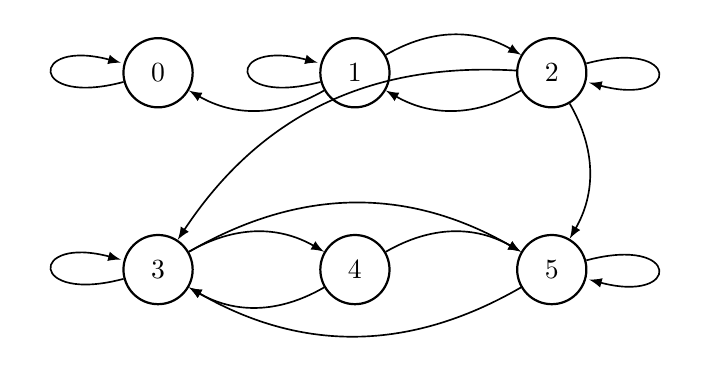
\begin{tikzpicture}[>=latex,scale=2.5,auto,semithick,node distance=3cm]
	\tikzstyle{every state}=[fill=white,draw=black,thick,text=black,scale=1]

	\tikzset{vertex/.style = {shape=circle,draw,minimum size=1.5em}}
	\tikzset{edge/.style = {->}}
	% vertices
	\node[state] (a) at  (0,1) {$0$};
	\node[state] (b) at  (1,1) {$1$};
	\node[state] (c) at  (2,1) {$2$};
	\node[state] (d) at  (0,0) {$3$};
	\node[state] (e) at  (1,0) {$4$};
	\node[state] (f) at  (2,0) {$5$};
	%edges
	\path (a) edge[->,loop left] (a);
	\path (b) edge[->,loop left] (b);
	\path (b) edge[->,bend left] (a);
	\path (b) edge[->,bend left] (c);
	\path (c) edge[->,bend left] (b);
	\path (c) edge[->,loop right] (c);
	\path (c) edge[->,bend right] (d);
	\path (c) edge[->,bend left] (f);


	\path (d) edge[->,loop left] (d);
	\path (d) edge[->,bend left] (e);
	\path (d) edge[->,bend left] (f);
	\path (e) edge[->,bend left] (f);
	\path (e) edge[->,bend left] (d);
	\path (f) edge[->,bend left] (d);
	\path (f) edge[->,loop right] (f);

	\end{tikzpicture}
	\end{center}

	Subsets of the graph with only incoming edges are closed.  Subsets
	of the graph where there is a path going through every element are 
	irreducible.  We therefore see the closed, irreducible subsets of the
	state space are $C_0=\{0\}$ and $C_1=\{3,4,5\}$.  Since these are
	finite, they must consist only of recurrent points.  We can also
	see that states $1$ and $2$ are not recurrent since there is a positive
	probability of transitioning into $C_0$ or $C_1$.

	\begin{theorem}
		Let $\mathcal S_R\subseteq \mathcal S$ be the set of all recurrent
		states for a Markov chain with state space $\mathcal S$.  Then
		$\mathcal S_R = \bigcup C_i$ where $\{C_i\}$ are disjoint, closed,
		and irreducible.
	\end{theorem}

	\begin{proof}
		Suppose $C$ is a closed set of recurrent points. Then $\ldsto$ is an equivalence
		relation on $C$.

		It is clear that since for any two states $x,y$, either $\rho_{xy}>0$ or $\rho_{xy}=0$,
		$\ldsto$ is a relation on the set of states.  We will now show it satisfies the properties
		of an equivalence relation.

		\begin{enumerate}
			\item[(reflexive)] If $x\in C$, then $x\ldsto x$ because $x$ is recurrent.
			\item[(symmetric)] If $x,y\in C$ and $x\ldsto y$, then $y\ldsto x$ by our second theorem.
			\item[(transitive)] If $x,y,z\in C$ and $x\ldsto y$ and $y\ldsto z$, then
				$\rho_{xz} \geq \rho_{xy}\rho_{yz} > 0$, so $x\ldsto z$.
		\end{enumerate}

		Now, notice that $\mathcal S_R$ is closed.  Suppose $y\notin \mathcal S_R$.  Then,
		\[
			1=\rho_{xx} \leq 1-\rho_{xy},
		\]
		and so $\rho_{xy}=0$ which is equivalent to $\mathcal S_R$ beging closed.  Now,
		let $\{C_i\}$ be the partition coming from the equivalence relation $\ldsto$.
	\end{proof}

\end{document}
